\section{Resultados y discuciones}

Los resultados se presentan a continuación en el orden en el que se emplean 
los pasos en la librería de Python \path{galpynostatic}: una primera subsección
para el preprocesamiento de los datos experimentales, luego otra para el ajuste
de estos datos con el modelo heurístco, y, por último, la utilización de este
para predecir las condiciones del tamaño de partícula pára lograr una carga
rápida en 15 minutos. Sumado a esto, también se comparan el comportamiento que
tendrían los distintos materiales, dados sus parámetros fundamentales, a 
distintos tamaños.

\subsection{Preprocesamiento de los datos experimentales}

Un procedimiento experimental usual para evaluar los materiales de las baterías
consiste en medir los perfiles galvanostáticos a distintos valores de C-rate.
En la Figura \ref{fig:preproc} se muestran como ejemplo las mediciones realizadas
por Wang \textit{et al.} \cite{wang2019high} para LiCoO$_2$ (LCO) recubierto con 
TiO$_2$. Además, se agrega una línea punteada horizontal que se corresponde
con el potencial de equilibrio reportado en el trabajo citado, 3.9 V, y otra
0.15 V por debajo, que es el valor que corresponde al potencial de corte
elegido en este capítulo. Esta es la región de interés en el gráfico, ya que 
los valores en los que el SOC se intersecta con esta última curva (SOC$_{\max}$)
son los que se utilizan para ajustar el modelo en función de C-rate.
\begin{figure}[h!]
    \centering
    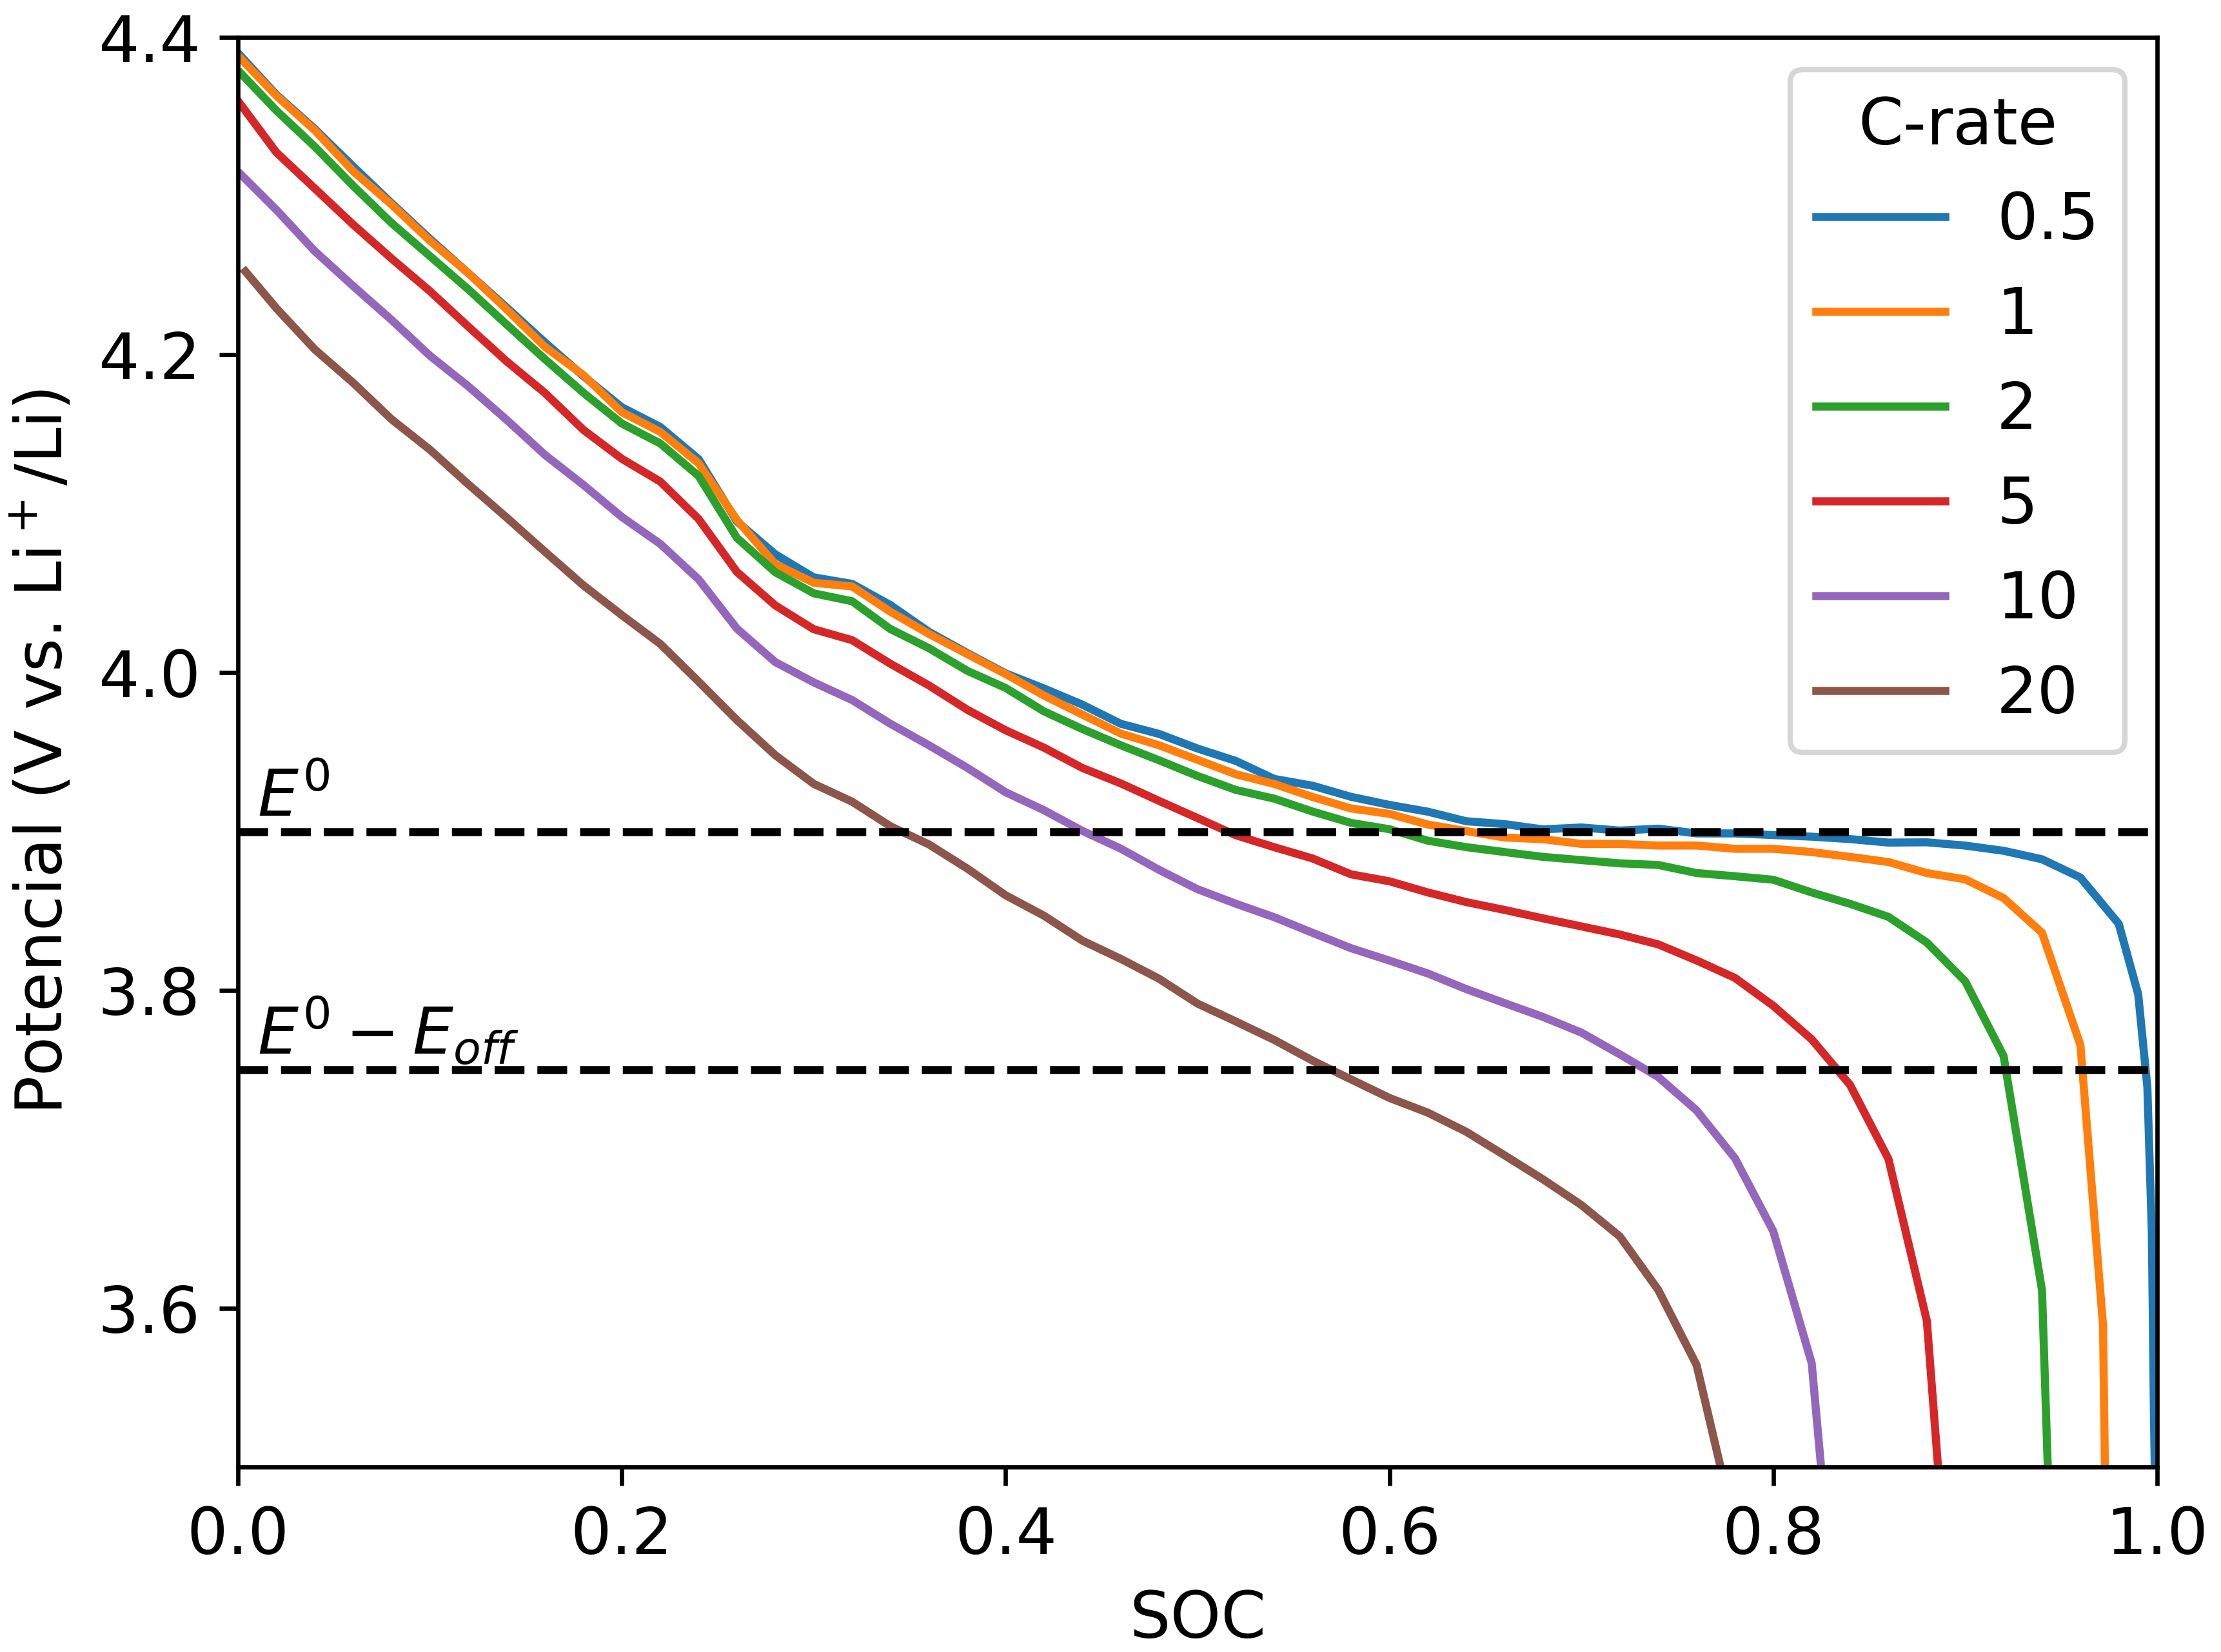
\includegraphics[width=0.7\textwidth]{FastCharging/un/resultados/preprocesamiento/preprocesamiento.png}
    \caption{Perfiles galvanostáticos para distintos valores de C-rate para el
    sistema LCO recubierto de TiO$_2$. Las líneas horizontales indican el 
    potencial de equilibrio y el de corte utilizado para determinar la 
    capacidad máxima normalizada alcanzada (SOC$_{\max}$) a cada C-rate. 
    Reproducido del trabajo de Wang \textit{et al.} \cite{wang2019high}.}
    \label{fig:preproc}
\end{figure}

Es importante destacar que, en el trabajo citado, los perfiles galvanostáticos
se presentan en función del SOC normalizado, que no siempre es el caso. La 
forma usual en la que estos resultados son reportados es en función de la 
capacidad de descarga. En estos casos, es necesario normalizarla con respecto
a la capacidad máxima ($Q_{\max}$) alcanzada por el material, para así obtener
el SOC normalizado. El criterio utilizado en este capítulo para encontrar 
$Q_{\max}$ fue considerar el valor máximo de la capacidad alcanzado por la 
medición a la C-rate más baja. Gráficos similares al presentado en la Figura 
\ref{fig:preproc} son obtenidos en el resto de los trabajos experimentales que
se utilizan en los ajustes que siguen.


% Copyright (c) 2024, Francisco Fernandez
% License: CC BY-SA 4.0
%   https://github.com/fernandezfran/thesis/blob/main/LICENSE
\subsection{Ajuste de dos conjuntos de parámetros DFTB}

Como fue introducido en la sección \ref{s:dftb}, para el método DFTB hay dos 
grupos de parámetros a ser determinados, los electrónicos (los orbitales 
pseudoatómicos y las densidades electrónicas) y los potenciales repulsivos para 
cada par de elementos químicos (Si-Si, Si-Li y Li-Li). La optimización de cada 
uno de ellos está sujeta a reproducir alguna propiedad deseada, como la 
estructura de bandas, las energías de atomización, entre otras. Para el ajuste
de la estructura de bandas se siguió el trabajo de van den Bossche \cite{van2019},
considerándose para el Li los electrones de valencia 2s mientras que para el Si 
los 3s y los 3p. La comparación de la estructura de bandas entre DFTB y DFT para 
los conjuntos A y B de parámetros se analiza en profundidad en la referencia 
\cite{oviedo2023}.

Para la parametrización del potencial de repulsión de cada uno de los conjuntos 
A y B se siguió el algoritmo de ajuste descripto en la sección \ref{s:algfit}
que permite optimizar los pesos de cada una de las estructuras en el conjunto de 
entrenamiento. Los coeficientes $\check{\boldsymbol{\xi}}_s$ minimizados para cada
conjunto, A y B, se reportan en la Tabla \ref{t:xiweights}.
\begin{table}[b]
    \centering
    \caption{Pesos óptimos, $\check{\boldsymbol{\xi}}_s$, de cada conjunto.}
    \setlength\extrarowheight{2pt}\stackon{%
    \begin{tabular}{l c c}
        \toprule
        \textbf{$s$} & 
        \textbf{conjunto A} & 
        \textbf{conjunto B} \\ 
        \midrule
        Li & $0.23\times10^{-2}$ & 0.49 \\
        Li$_{15}$Si$_4$ & 0.15 & 0.28$\times10^{-21}$ \\
        Li$_{13}$Si$_4$ & 0.21 & 0.17$\times10^{-1}$ \\
        Li$_7$Si$_3$ & 0.21 & 0.11$\times10^{-1}$ \\
        Li$_{12}$Si$_7$ & 0.23 & 0.11$\times10^{-2}$ \\
        LiSi & 0.21 & 0.35$\times10^{-3}$ \\
        Si & 0.83$\times10^{-7}$ & 0.49 \\
        \bottomrule
    \end{tabular}
    }{}
    \label{t:xiweights}
\end{table}
Es interesante que para el conjunto A el algoritmo reduce los pesos relativos del 
Li y del Si puro y aumenta los de las aleaciones. Mientras que para el conjunto 
B sucede lo contrario, los pesos óptimos son mayores para los elementos puros y
menores para las aleaciones. Este comportamiento se debe a que el término de la 
energía de bandas del conjunto A se construye utilizando los elementos puros 
mientras que el mismo término para el conjunto B utiliza una de las aleaciones. 
Resulta razonable que el término de repulsión, que busca compensar el residuo de la 
energía dada por todas las demás contribuciones energéticas, sea menos importante 
para las estructuras consideradas en el ajuste de las energías de banda y más 
importante para el resto. Así, los coeficientes óptimos $\check{\boldsymbol{\xi}}_s$ 
parecen ser capaces de percibir esta situación y tratar de compensarla al centrar 
la parametrización en las estructuras que más la necesitan.

Otra observación que surge de la Tabla \ref{t:xiweights} es el peso relativo bajo
que resulta en ambos conjuntos para la aleación cristalina Li$_{15}$Si$_4$, en 
comparación con el resto de las aleaciones. En particular, para el conjunto B este 
peso es prácticamente igual a cero, indicando que la inclusión de estas 
estructuras en el conjunto de entrenamiento no contribuye a una mejora de la 
predicción de las energías de formación relativas. Esto puede deberse a que la 
estructura de Li$_{15}$Si$_4$ tiene una naturaleza particular que difiere del 
resto de las aleaciones e interfiere de alguna manera con el ajuste de los 
parámetros del modelo. Por ejemplo, una explicación posible puede ser que el 
entorno químico de esta estructura es bastante diferente al del resto de las 
aleaciones por lo que la predicción global puede ser mejorada al centrar el 
ajuste en el resto de las aleaciones. En este sentido, el procedimiento de 
optimización propuesto en este capítulo puede considerarse como una herramienta 
para detectar peculiaridades dentro del conjunto de entrenamiento.

